\chapter{Ελληνική Μετάφραση}
\label{appendices:greek}

Εδώ θα παραθέσουμε μια εκτενή περίληψη της παρούσας εργασίας στα ελληνικά.


\section{Εισαγωγή}
Το Pidgin είναι μια διαδεδομένη εφαρμογή desktop για συνομιλίες πραγματικού χρόνου.
Συνοδεύεται από το OTR πρόσθετο το οποίο, χρησιμοποιώντας το OTR πρωτόκολλο \cite{otr} \cite{otr_improvedauth} \cite{otr_userstudy}, προσθέτει στο Pidgin τη δυνατότητα των από άκρο σε άκρο κρυπτογραφημένων συνομιλιών μεταξύ δύο ατόμων.
Έτσι προσφέρει ασφαλείς συνομιλίες στις οποίες μόνο οι συνδιαλεγόμενοι μπορούν να διαβάσουν τα μηνύματα που ανταλλάσσονται, τα οποία είναι κρυφά ακόμα και στον πάροχο επικοινωνίας.
Παρότι το ίδιο το OTR πρόσθετο προσφέρει συνομιλίες μόνο δύο ατόμων, τα υποβόσκωντα πρωτόκολλα συχνά παρέχουν "δωμάτια" πολλών χρηστών, όπου πολλοί μπορούν να συνομιλούν ταυτόχρονα μεταξύ τους.
Μέχρι τώρα όσοι μιλούσαν σε τέτοιου είδους δωμάτια δεν απολάμβαναν τα πλεονεκτήματα της από άκρο σε άκρο κρυπτογράφησης.

Στόχος της εργασίας μας είναι η υλοποίηση μιας βιβλιοθήκης για ασφαλείς συνομιλίες μεταξύ πολλών ατόμων.
Επιπρόσθετα υλοποιούμε κι ένα πρόσθετο για το Pidgin το οποίο χρησιμοποιεί αυτή τη βιβλιοθήκη έτσι ώστε να επιτρέπει τους χρήστες του Pidgin να συνομιλούν ασφαλώς σε ένα οικείο περιβάλλον.

Η δουλειά μας βασίζεται θεμελιωδώς στο mpOTR paper \cite{mpotr}.
Ακολουθώντας τις συμβάσεις του OTR πρωτοκόλλου, ο όρος "ιδιωτικός" χρησιμοποιείται για να περιγράψει τις ιδιότητες των συνομιλιών της πραγματικής ζωής:

\begin{itemize}
  \item Εμπιστευτικότητα\\
    Μόνο οι συμμετέχοντες μπορούν να διαβάσουν τα μηνύματα\\[0.2cm]

  \item Αυθεντικοποίηση\\
    Οι συμμετέχοντες είναι βέβαιοι ότι πραγματικά μιλάνε σε αυτούς που νομίζουν ότι μιλάνε\\[0.2cm]

  \item Διαψευσιμότητα\\
    Κανείς δε μπορεί να αποδείξει σε κάποιον που δε συμμετείχε στη συνομιλία, ότι κάποιο συγκεκριμένος συμμετέχοντας έλαβε μέρος στη συνομιλία αυτή\\[0.2cm]

  \item Προώθηση Μυστικότητας\\
    Εάν τα μακροπρόθεσμα μυστικά ενός χρήστη εκτεθούν σε κάποιον επιτιθέμενο, τότε αυτός δε μπορεί να διαβάσει κανένα μήνυμα το οποίο στάλθηκε παλαιότερα\\[0.2cm]

\end{itemize}

Όταν έχουμε να κάνουμε για συνομιλίες πολλών ατόμων, μια ακόμα ιδιότητα απαιτείται.
Αυτή η ιδιότητα λέγεται συνέπεια περιεχομένων δωματίου, και γενικά δηλώνει ότι όλοι οι συμμετέχοντες έχουν την ίδια εικόνα για τα μηνύματα που έχουν σταλθεί σε κάποιο δωμάτιο.

Για να υλοποιήσουμε το mpOTR πρωτόκολλο το οποίο περιγράφεται στο \cite{mpotr}, έπρεπε να συγκεκριμενοποιήσουμε τα υπο-πρωτόκολλα τα οποία χρησιμοποιούταν ως μαύρα κουτιά και δεν περιγράφηκαν πλήρως.
Προτείνουμε μια συγκεκριμένη Διαψεύσιμη Ανταλλαγή Κλειδιών Υπογραφής (DSKE) η οποία βασίζεται σε εκτέλεση κατά ζεύγη του τριπλού \dhname πρωτοκόλλου.
Για την Ομαδική Συμφωνία Κλειδιού (GKA) χρησιμοποιούμε το πρωτόκολλο που περιγράφεται στο \cite{mpenc}, αλλά χρησιμοποιούμε κλασσικό \dhname (δηλαδή όχι \dhname ελλειπτικών καμπυλών).

Υλοποιούμε την mpOTR βιβλιοθήκη ως κομμάτι της αρχικής OTR βιβλιοθήκης όπως φαίνεται στο \href{https://github.com/Mandragorian/libotr/tree/mpotr}{το github repo μας\footnote{https://github.com/Mandragorian/libotr/tree/mpotr}}, η οποία μέχρι τώρα πρόσφερε συνομιλίες μόνο για δύο συμμετέχοντες.
Το πρόσθετο μας βασίζεται στο ήδη υπάρχον OTR πρόσθετο το οποίο αναπτύσσεται από την κοινότητα του OTR, και μπορεί κανείς να το δει στο \href{https://github.com/Mandragorian/pidgin_otr/tree/mpotr_integration}{το github repo μας\footnote{https://github.com/Mandragorian/pidgin\_otr/tree/mpotr\_integration}}.
%------------------------------------------------

\section{Το Πρωτόκολλο}
\begin{algorithm}[h]
  \KwIn{$\mathcal{P}$ : participants list}
	\KwResult{Executes a run of the mpOTR protocol}
	\Begin{

  $sid$ := Offer($\mathcal{P}$)

  $\mathcal{S}$ := DSKE($sid$, $\mathcal{P}$)

  $\mathcal{K}$ := GKA($sid$, $\mathcal{S}$, $\mathcal{P}$)

  $A$ := Attest($sid$, $\mathcal{S}$, $\mathcal{P}$)

  \If{$A$ $\ne$ "OK"}{
    \Return{"Error"}
  }

  $\mathcal{T}$ := Communication($sid$, $\mathcal{K}$, $\mathcal{S}$, $\mathcal{P}$)

  $consensus$ := Shutdown($sid$, $\mathcal{T}$, $\mathcal{S}$, $\mathcal{P}$)

  \If{$consensus$ = "consensus"}{
    \Return{"OK"}
  }
  \Else{
    \Return{"Error"}
  }

	}
	\caption{The mpOTR protocol}
	\label{mpotr_algo}
\end{algorithm}

Στον αλγόριθμο \ref{mpotr_algo} παρουσιάζουμε τη συμπεριφορά του πρωτοκόλλου.
Το πρωτόκολλο χωρίζεται σε διάφορες φάσεις τις οποίες ονομάζουμε υπο-πρωτόκολλα.
Τα τέσσερα πρώτα από αυτά (Offer, DSKA, GKA και Attest) είναι υπεύθυνα για να κατασκευάσουν όλη την απαραίτητη πληροφορία που απαιτείται ώστε να λάβει χώρα μια ιδιωτική συνομιλία.
Το Communication υπο-πρωτόκολλο είναι αυτό το οποίο αναλαμβάνει να φέρει εις πέρας την ίδια τη συνομιλία.
Τέλος το Shutdown υπο-πρωτόκολλο είναι υπεύθυνο ώστε να γίνει κάθε απαιτούμενη ενέργεια που πρέπει να συμβεί πριν κλείσει μια συνομιλία.
Παρουσιάζουμε εν συντομία τα υπο-πρωτόκολλα αυτά παρακάτω.

Κατά τη διάρκεια του Offer υπο-πρωτοκόλλου, οι συμμετέχοντες υπολογίζουν ένα αναγνωριστικό $sid$ για τη συνομιλία.
Αυτό είναι ένας αριθμός, μοναδικός με μεγάλη πιθανότητα, που ταυτοποιεί τη συνομιλία.

Κατά το DSKE υπο-πρωτόκολλο, κάθε συμμετέχοντας κατασκευάζει έναν πίνακα αντιστοίχησης $\mathcal{S}$ ο οποίος αντιστοιχεί κάθε συμμετέχοντα σε ένα κλειδί υπογραφής το οποίο θα χρησιμοποιηθεί γι αυτή τη συνομιλία.
Κάθε συμμετέχοντας παράγει ένα εφήμερο κλειδί υπογραφής με το οποίο θα αυθεντικοποιεί τα μηνύματά του.
Έπειτα κάθε συμμετέχοντας στέλνει το δημόσιο κομμάτι του κλειδιού υπογραφής του με κάθε άλλο συμμετέχοντα, χρησιμοποιώντας μια Διαψεύσιμη Αυθεντικοποιημένη Ανταλλαγή Κλειδιού (DAKE).
Όταν όλοι έχουν ανταλλάξει τα κλειδιά τους με όλους ο κάθε συμμετέχοντας έχει κατασκευάσει τον πίνακα αντιστοίχισης του.
Αφού η ανταλλαγή κλειδιού είναι διαψεύσιμη, το ίδιο ισχύει και για τα κλειδιά υπογραφής.
Θα μιλήσουμε πιο αναλυτικά για το DSKE και το DAKE στην παράγραφο (\ref{dske_subprot}).

Κατά το GKA υπο-πρωτόκολλο, οι συμμετέχοντες παράγουν ένα κοινό κλειδί $\mathcal{K}$ το οποίο θα χρησιμοποιηθεί για να παραχθούν κλειδιά κρυπτογράφησης.
Τα κλειδιά αυτά θα χρησιμοποιηθούν για να κρυπτογραφηθούν τα μηνύματα που θα σταλούν κατά τη συνομιλία.
Το υπο-πρωτόκολλο αυτό περιγράφεται αναλυτικότερα στην παράγραφο (\ref{gka_subprot}).

Κατά το Attest υπο-πρωτόκολλο οι συμμετέχοντες αυθεντικοποιούν το αναγνωριστικό $sid$ και σιγουρεύονται ότι έχουν φτάσει στον ίδιο πίνακα αντιστοίχισης κλειδιών υπογραφής $\mathcal{S}$.

Κατά το Communication υπο-πρωτόκολλο, λαμβάνει χώρα η ίδια η συνομιλία.
Οι χρήστες χρησιμοποιούν το κοινό μυστικό $\mathcal{K}$, τα εφήμερα κλειδιά υπογραφής και τον πίνακα αντιστοίχισης $\mathcal{S}$, ώστε να κρυπτογραφήσουν και να αυθεντικοποιήσουν τα μηνύματά τους.
Όταν τελειώσει αυτή η φάση παράγεται ένα αντίγραφο της συνομιλίας το οποίο περιέχει όλα τα μηνύματα της συνομιλίας.

Κατά το Shutdown υπο-πρωτόκολλο, οι συμμετέχοντας αποφασίζουν αν υπάρχει συνέπεια περιεχομένων δωματίου και αποκαλύπτουν τα ιδιωτικά κομμάτια των κλειδιών υπογραφής τους.
Εάν τα περιεχόμενα είναι όντως συνεπή τότε λέμε ότι υπάρχει ομοφωνία.
Η αποκάλυψη των ιδιωτικών κλειδιών υπογραφής προσθέτει επιπλέον διαψευσιμότητα στο πρωτόκολλο, όπως και η αποκάλυψη των MAC κλειδιών στο OTR πρωτόκολλο.
Παρόλα αυτά είναι προαιρετικό βήμα καθώς το πρωτόκολλο που προτείνεται είναι διαψεύσιμο και χωρίς την αποκάλυψη.

\section{Τα υπο-πρωτόκολλα}
\label{subprots}

Εδώ θα παρουσιάσουμε τα δύο υπο-πρωτόκολλα τα οποία δεν περιγράφονται στο \cite{mpotr}, δηλαδή τη Διαψεύσιμη Ανταλλαγή Κλειδιών Υπογραφής και την Ομαδική Συμφωνία Κλειδιού.

\subsection{DSKE}
\label{dske_subprot}

In \cite{mpotr} the DSKE is partially described using a sub-sub-protocol named Deniable Authenticated Key Exchange (DAKE) as a black box.
In our implementation we use the Triple Diffie--Hellman key exchange as a DAKE.
Triple DH is an authenticated and deniable key exchange.

Each participant executes a Triple DH key exchange with every other participant in the chat room and they generate a shared secret.
Using that secret the user encrypt-then-MACs the public part of his signing key and sends it to the other participant.

After all participants have exchanged signing keys with each other in the manner stated above, they all have a signing key association table $\mathcal{S}$.
Note that the DSKE is the only step in the setup phase where $O(n^2)$ messages must be sent.
In the other setup phases and the communication phase only $O(n)$ messages are sent.

A schematic description of the protocol can be seen in figure \ref{den_ake_schematic}.

\begin{figure}[h]
  \fbox{%
    \pseudocode{%
      \textbf{Alice} \< \< \textbf{Bob} \\[][\hline]
      x \sample Z_p^* \< \< \\
      \< \sendmessageright*{Send \ \left(g^x,g^X\right)} \< \\
      \< \< y \sample Z_p^* \\
      \< \< s \leftarrow g^{xy} \Vert g^{Xy} \Vert g^{Yx} \\
      \< \< k_1 \leftarrow KDF_1(s) \\
      \< \< k_2 \leftarrow KDF_2(s) \\
      \< \sendmessageleft*{Send \ \left(g^y,g^Y\right)} \< \\
      s \leftarrow g^{xy} \Vert g^{Xy} \Vert g^{Yx} \< \< \\
      k_1 \leftarrow KDF_1(s) \< \< \\
      k_2 \leftarrow KDF_2(s) \< \< \\
      \< \sendmessageright*{ Send \\ c = AES_{k_1}("confirm") \\ MAC_{k_2}(c)\ } \< \\
      \< \< \text{Verify mac} \\
      \< \< m \leftarrow AES^{-1}_{k_1}(c) \\
      \< \< \text{Verify m = "confirm"} \\
      \< \sendmessageleft*{ Send \\ c = AES_{k_1}("confirm") \\ MAC_{k_2}(c)\ } \< \\
      \text{Verify mac} \< \< \\
      m \leftarrow AES^{-1}_{k_1}(c) \< \< \\
      \text{Verify m = "confirm"} \\
      \< \sendmessageright*{Send \\ c = AES_{k_1}(E_{\hat{A}}) \\ MAC_{k_2}(c) } \< \\
      \< \< \text{Verify mac} \\
      \< \< S[\hat{A}] \leftarrow E_{\hat{A}} \\
      \< \sendmessageleft*{Send \\ c = AES_{k_1}(E_{\hat{B}}) \\ MAC_{k_2}(c) } \< \\
      \text{Verify mac} \< \<  \\
     S[\hat{B}] \leftarrow E_{\hat{B}} \< \< \\
    }
  }

    \caption{The messages exchanged between two users in order to authenticate each other's signing keys. $X$ and $Y$ are the private parts of the long term keys. $KDF_1$ and $KDF_2$ are two key derivation functions.}
  \label{den_ake_schematic}
\end{figure}

\subsection{GKA}
\label{gka_subprot}

\begin{figure}
  \begin{minipage}{0.49\textwidth}
    \begin{tikzpicture}[scale=.9]
      \def \n {5}
      \def \ndec {4}
      \def \radius {3cm}
      \def \margin {8} % margin in angles, depends on the radius

      \foreach \s in {1,...,\ndec}
      {
        \node[draw, circle] at ({180 + (360/\n * (\s - 1))}:\radius) {$\s$};
        \draw[->, >=latex] ({145 + 36 + (360/\n * (\s - 1))+\margin}:\radius)
          arc ({145 + 36 + (360/\n * (\s - 1))+\margin}:{145 + 36 + 360/\n * (\s)-\margin}:\radius);
      }
      \node[draw, circle] at ({181 + 360/\n * (\n - 1)}:\radius) {$\n$};
    \end{tikzpicture}
    \caption{This diagram demonstrates the upflow of the intermediate keys}
    \label{upflow_diagr}
  \end{minipage}
  \begin{minipage}{0.49\textwidth}
    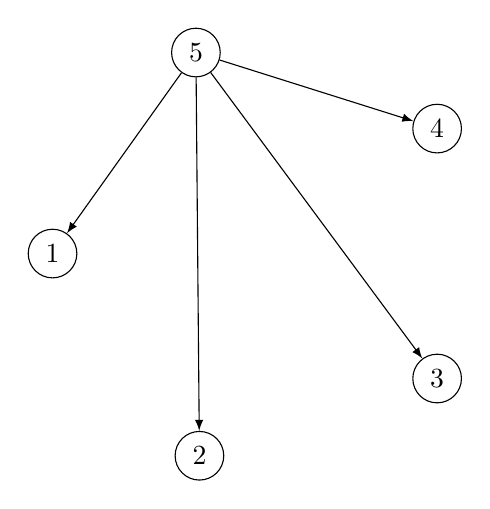
\begin{tikzpicture}[scale=.9]
      \def \n {5}
      \def \ndec {4}
      \def \radius {3cm}
      \def \margin {8} % margin in angles, depends on the radius

      \foreach \s in {1,...,\ndec}
      {
        \node[draw, circle](\s) at ({180 + (360/\n * (\s - 1))}:\radius) {$\s$};
      }
      \node[draw, circle](5) at ({181 + 360/\n * (\n - 1)}:\radius) {$\n$};
      \draw[->, >=latex] (5) -- (1);
      \draw[->, >=latex] (5) -- (2);
      \draw[->, >=latex] (5) -- (3);
      \draw[->, >=latex] (5) -- (4);
    \end{tikzpicture}
    \caption{This diagram demonstrates the downflow of the intermediate keys}
    \label{downflow_diagr}
  \end{minipage}
\end{figure}

For a GKA we use the protocol as specified in \cite{mpenc}.
Again, the basic idea used here is the Diffie--Hellman key exchange generalized for many participants.

During the GKA protocol, messages are exchanged in two phases: The upflow and the downflow phase.
During the upflow phase, the messages are exchanged between participants in a sequential manner, and each next participant calculates keys based on the accumulated messages received from the previous participant before contacting the next participant, as shown in Figure \ref{upflow_diagr}.
After the completion of the upflow phase, the last participant has collected enough data for key generation.
This data is subsequently communicated to the rest of the group during the downflow phase, as shown in Figure \ref{downflow_diagr}.

In algorithms \ref{upflow_algo}, \ref{downflow_algo}, \ref{gka_proto_algo} the main idea of the GKA we use is presented.

\begin{algorithm}[h]
	\KwIn{P : participants list}
	\KwIn {InterKeys : previous intermediate key list}
	\KwIn {X : user's secret key}
	\KwIn {N : next participant}
	\KwResult{Sends the new intermediate key list to the next participant}
	\Begin{
	inter\_key\_list := empty\_list

	inter\_key\_list.append( InterKeys.last\_elem() )

	\ForEach{k in InterKeys}
	{
		inter\_key\_list.append( $k^X$ )
	}

	send( N , P || inter\_key\_list)
	}
	\caption{Upflow Message send algorithm, send\_upflow}
	\label{upflow_algo}
\end{algorithm}

\begin{algorithm}
	\KwIn{P : participants list}
	\KwIn {InterKeys : previous intermediate key list}
	\KwIn {X : user's secret key}
	\KwIn {N : next participant}
	\KwResult{Sends the downflow intermediate key list to the other participants}
	\Begin{
	inter\_key\_list := empty\_list

	\ForEach{k in InterKeys}
	{
		inter\_key\_list.append( $k^X$ )
	}

	inter\_key\_list.reverse()

	Broadcast( P || inter\_key\_list)
	}
	\caption{Downflow Message send algorithm, send\_downflow}
	\label{downflow_algo}
\end{algorithm}

\begin{algorithm}[h]
	\KwIn{P : participants list}
	\KwOut{The shared secret}
	\KwResult{Executes a GKA and produces the shared secret}
	\Begin{

	prev := get\_previous\_participant()

	next := get\_next\_participant()

	x := gka\_genkey()

	\If{prev == NULL}{
		send\_upflow(P, [G], x, next)
		}
	\Else{
			m = receive\_from(prev)

			\If{ m not valid}{
					return error
			}
			\If{ next != NULL}{
				send\_upflow(P, m.key\_list, x, next)
			}
			\Else{
				final\_key := m.key\_list.last\_elem()

				s := $final\_key^x$

				send\_downflow(P, m.key\_list, x)

				return s
			}
	}

	m = wait\_for\_downflow()

	\If{m not valid}{
		return error
	}

	final\_key := m.key\_list[pos]

	s := $final\_key^x$

	return s

	}
	\caption{The GKA protocol}
	\label{gka_proto_algo}
\end{algorithm}

\section{The primitives}

\subsection{Diffie--Hellman Group}
The already existing libotr implementation of the DH key exchange is used.
As a result we use classic Diffie--Hellman , and specifically the group no. 5 \cite{website:dh-rfc} with a 1536 bit modulus.
In the algorithms presented above, all exponentiations are performed in this group.

\subsection{Encryption}
For encryption we use AES-128 in CTR mode, the same cipher as the two-party OTR protocol.
We chose 128-bit AES instead of the 256-bit one because our Diffie--Hellman group does not provide 256 bit of entropy and evidence suggests that the 128-bit AES key schedule is preferred for security \cite{aes-key-recov} \cite{rijndael-improved-analysis}.

To encrypt a message, a user concatenates the shared secret with his personal id and creates a personal key.
This is the actual encryption key.
\[
k_{enc} = H(id_{personal} || master\ key)
\]
For the counter, each user stores locally his personal upper half (8 most significant bytes).
The lower half (8 least significant bytes) are always set to zero.
The top half of the counter is prepended in the sent message.
The ciphertext is produced as follows (where $ctr$ is the top half of the locally stored counter):

\[
ciphertext = AES_{CTR}(k_{enc}, ctr||0, plaintext)
\]

To decrypt a message, a user concatenates the shared secret with the id of the message's sender.
\[
k_{dec} = H(id_{sender} || master\ key)
\]
He uses the prepended top half of the counter.

\[
plaintext = AES_{CTR}(k_{dec}, ctr||0, ciphertext)
\]

This encryption scheme is used, so that the possibility that a certain encryption key and counter pair is eliminated.
If all the participants used the shared secret itself as an encryption key and two users sent a message at the same time, they would use the same counter.
This would be a catastrophic failure.

\subsection{Authentication}
For signing we use the EdDSA algorithm over the Ed25519 curve.
This signature scheme was chosen primarily because of its fast key generation.
Each message is signed as a whole.
This means that the signature covers the message and any metadata sent, like session id, counter value etc.
